\chapter{Experiments}
\label{chap:experiments}
	\textit{This chapter discusses the division of the data set before training, assessment techniques, and experimental results. Compare the outcomes of the experiments we suggest to the reference experiments from relevant works.}
\minitoc

\section{Data preparation} 
\label{sec:data_preparation}
	Đối với các giải thuật học máy nói chung cũng như mạng học sâu nói riêng, việc chuẩn bị dữ liệu là vô cùng quan trọng. Nếu sử dụng mô hình đã huấn luyện để dự đoán trên tập dữ liệu không cùng phân bố với tập dữ liệu được sử dụng để huấn luyện mô hình trước đó thì kết quả dự đoán không thể chính xác. Do đó, phân chia dữ liệu sao cho phân bố trên các tập đồng đều với nhau là một trong những yếu tố quan trọng quyết định tới mức hiệu quả của mạng học sâu. 
	
	Sau khi khảo sát các ảnh chụp CT của 20 bệnh nhân, chúng tôi nhận thấy sự xuất hiện các khối u có ảnh đưởng đến phân phối mức sáng của các điểm ảnh trong cơ quan gan. Do đó, chúng tôi chia các bệnh nhân ra 03 nhóm: bệnh nhân không có khối u trong gan, bệnh nhân có một khối u trong gan và bệnh nhân có nhiều khối u trong gan. Chúng tôi chia tập dữ liệu thành ba tập dữ liệu bao gồm tập huấn luyện, tập kiểm thử và tập kiểm tra sao cho mỗi tập đều có bệnh nhân không có u, bệnh nhân có một khối u và bệnh nhân có nhiều khối u. Chi tiết các tập dữ liệu được chúng tôi trình bày trong \autoref{tab:3d_ircadb_01_division}.
	\begin{table}[h!]
		\centering
		\caption{Bảng phân chia các bệnh nhân thành các tập dữ liệu.}
		\label{tab:3d_ircadb_01_division}
		\begin{tabular}{@{\hspace{4mm}}c@{\hspace{5mm}}ll@{\hspace{9mm}}l@{\hspace{9mm}}lr@{\hspace{5mm}}}
			\toprule
			\multirow{2}{*}{\textbf{STT}} & \multirow{2}{*}{\textbf{Tập}} & \multicolumn{3}{c}{\textbf{Số lượng khối u gan}} & \multirow{2}{*}{\textbf{\ \ Tổng}} \\ \cmidrule(l){3-5}
			&  & \textbf{0 khối u} & \textbf{1 khối u} & \textbf{Nhiều khối u} &  \\ \midrule
			1 & Huấn luyện\ \ \ & 5, 7, 11 & 2, 3, 9, 12 & 1, 4, 8, 10, 15, 17, 19 & 14 \\[1mm]
			2 & Kiểm thử & 14 & 16 & 6 & 3 \\[1mm]
			3 & Kiểm tra & 20 & 18 & 13 & 3 \\ \bottomrule
		\end{tabular}
	\end{table}

\section{Evaluation methods} 
\label{sec:evaluation}
	Quá trình đánh giá một mô hình phân đoạn hình ảnh y khoa liên quan đến việc đánh giá độ chính xác của kết quả dự đoán. Hai hoạt động cơ bản cần được tiến hành để đánh giá một cách toàn diện một mô hình là đánh giá định tính và đánh giá định lượng. Đánh giá định lượng cho biết một cách tổng quát độ tốt của mô hình, trong khi đó đánh giá định tính cho biết mức độ ổn định của mô hình trong quá trình làm việc (trong trường hợp xấu nhất, trung bình và tốt nhất). Trong phần này, chúng tôi trình bày 4 độ đo có liên quan bao gồm Precision, Recall, IoU và Dice. Trong đó, IoU và Dice được chúng tôi sử dụng để đánh giá kết quả dự đoán của các mô hình.
\newpage
	Ta quy ước,
	\begin{itemize}
		\item TP (true positive): số lượng điểm ảnh foreground\index{Foreground} được dự đoán đúng,
		\item TN (true negative): số lượng điểm ảnh background\index{Background} được dự đoán đúng,
		\item FP (false positive): số lượng điểm ảnh background bị dự đoán sai,
		\item FN (false negative): số lượng điểm ảnh foreground bị dự đoán sai.
	\end{itemize}
	\begin{description}
		\item[Precision] trả lời cho câu hỏi ``Số dự đoán thực sự chính xác chiếm bao nhiêu phần trong số các dự đoán foreground?''. Công thức Precision được định nghĩa trong \autoref{eqn:precision}. Precision càng cao, kết quả dự đoán càng tốt.
		\begin{equation}
		Precision = \dfrac{TP}{TP + FP} \label{eqn:precision}
		\end{equation}
		
		\item[Recall] trả lời cho câu hỏi ``Số dự đoán thực sự chính xác chiếm bao nhiêu phần trong số các mẫu foreground''. Công thức Recall được định nghĩa trong \autoref{eqn:recall}. Recall càng cao, kết quả dự đoán càng tốt.
		\begin{equation}
		Recall = \dfrac{TP}{TP + FN} \label{eqn:recall}
		\end{equation}
		
		\item[Dice] là độ đo cân bằng giữa Precision và Recall. Trong trường hợp mô hình dự đoán chính xác một lượng nhỏ mẫu thuộc foreground, giá trị Precision sẽ cao, tuy nhiên số lượng false negative sẽ cao theo, nghĩa là giá trị Recall thấp. Trong trường hợp mô hình dự đoán một lượng lớn mẫu thuộc foreground, giá trị Recall sẽ cao, tuy nhiên số lượng false positve sẽ cao theo, tức là giá trị Precision thấp. Dice được tính toán bằng cách sử dụng đồng thời Precision và Recall. Khi giá trị Precision và giá trị Recall cùng cao, giá trị Dice sẽ cao, ngược lại, khi một trong hai giá trị Precision và Recall thấp, giá trị Dice sẽ thấp. Do đó, Dice phù hợp cho các bài toán phân loại có sự mất cân bằng về nhãn. Công thức Dice được định nghĩa trong \autoref{eqn:recall}.
		\begin{equation}
		Dice = 2 * \dfrac{Precision * Recall}{Precision + Recall}
		\end{equation}
		\item[IoU\nomenclature{IoU}{Intersection over Union}] cho biết mức độ tương tự giữa hai mẫu $X$ và $Y$. IoU được định nghĩa trong \autoref{eqn:iou}.
		\begin{equation}
		IoU = \dfrac{|X \cap Y|}{|X| + |Y| - |X \cap Y|} \label{eqn:iou}
		\end{equation}
	\end{description}

	
\newpage
\section{Experiment results} 
\label{sec:exp_results}
	Trước khi tiến hành các thí nghiệm để đánh giá hệ thống, chúng tôi thực hiện kiểm chứng tính hiệu quả của đề xuất cắt giảm độ sâu trong mô hình U-Net, để từ đó chọn ra mô hình tốt hơn phục vụ cho các thí nghiệm về sau. \autoref{tab:dac_ta_sieu_tham_so_thi_nghiem_unet_va_unet_star} đặc tả thông số chi tiết của các thí nghiệm dùng để so sánh tính hiệu quả trước và sau điều chỉnh số tầng ở mô hình U-Net sử dụng convolution 3D.
	\begin{table}[h!]
		\caption{Thông số các thí nghiệm so sánh tính hiệu quả trước và sau điều chỉnh số tầng ở mô hình U-Net sử dụng convolution 3D.}
		\label{tab:dac_ta_sieu_tham_so_thi_nghiem_unet_va_unet_star}
		\resizebox{\columnwidth}{!}{
			\begin{tabular}{clcllrr}
				\toprule
				\textbf{STT} & \textbf{Kiến trúc} & \textbf{Số tầng}     & \textbf{BatchNorm\index{Batchnorm}} & \textbf{Hàm lỗi} & \textbf{Learning rate\index{Learning rate}} & \textbf{Momentum}     \\ \midrule
				1            & U-Net        & 5 			& Không 			 & CrossEntropy     & 0.0001          		 & 0.90 \\
				2            & U-Net*        & 3 					& Không 			 & CrossEntropy     & 0.0001          		 & 0.90 \\
				\bottomrule
			\end{tabular}
		}
	\end{table}

	\autoref{tab:so_sanh_unet_3_va_5_tang} là kết quả thu được khi so sánh hai mô hình. Từ kết quả này chúng ta thấy rằng, chất lượng phân đoạn hệ thống mạch máu trên tập kiểm tra trước và sau hậu xử lý (cột \textbf{Tập kiểm tra} và \textbf{Tập kiểm tra*}) ở mô hình U-Net* không có nhiều sự khác biệt so với mô hình U-Net. Chứng tỏ, việc cắt giảm hai tầng 4 và 5 trong mô hình U-Net là hợp lý vì chúng không có nhiều đóng góp trong quá trình học. Hơn nữa, việc cắt giảm số tầng giúp cho mô hình trở nên nhẹ hơn, thời gian inference\index{Inference}\footnote{Inference trong lĩnh vực học sâu là thuật ngữ dùng để chỉ giai đoạn mô hình sau huấn luyện được sử dụng để dự đoán các mẫu dữ liệu thử nghiệm. Không giống quá trình huấn luyện, inference không thực hiện lan truyền ngược để tính toán lỗi và cập nhật trọng số.}trung bình cho một tập ảnh CT ở mô hình U-Net* là 4.46 giây, nhanh hơn gần 1 giây so với mô hình U-Net là 5.40 giây. Chênh lệch này tuy nhỏ nhưng sẽ có ý nghĩa rất lớn khi áp dụng mô mình vào thực tiễn với khối lượng dữ liệu khổng lồ. Thời gian dành cho công tác chẩn đoán càng được rút ngắn bao nhiêu, cơ hội chữa trị thành công cho bệnh nhân càng lớn bấy nhiêu. Vì vậy, chúng tôi lựa chọn sử dụng mô hình U-Net* trong các thí nghiệp về sau để đánh giá hệ thống.
	\begin{table}[h!]
		\caption{Kết quả so sánh tính hiệu quả trước và sau điều chỉnh số tầng ở mô hình U-Net sử dụng convolution 3D.}
		\label{tab:so_sanh_unet_3_va_5_tang}
		\resizebox{\columnwidth}{!}{
			\begin{tabular}{clcccccc}
				\toprule
				\multicolumn{1}{c}{\multirow{2}{*}{\textbf{\ \ STT\ }}} & \multicolumn{1}{l}{\multirow{2}{*}{\textbf{Kiến trúc}}} & \multicolumn{1}{c}{\multirow{2}{*}{\textbf{Thời gian inference (s)\ \ }}} & \multicolumn{2}{c}{\textbf{Tập kiểm tra}} & & \multicolumn{2}{c}{\textbf{Tập kiểm tra*}} \\ \cmidrule{4-5} \cmidrule{7-8} 
				\multicolumn{1}{l}{} & \multicolumn{1}{l}{} & \multicolumn{1}{l}{} & \textbf{IoU} & \textbf{Dice} & \multicolumn{1}{l}{} & \textbf{IoU} & \textbf{Dice} \\ \midrule
				1 & U-Net & 5.40 & 0.365 & 0.533 & & 0.379 & 0.548 \\
				2 & U-Net* & 4.46 & 0.380 & 0.550 & & 0.375 & 0.545 \\
				\bottomrule
			\end{tabular}
		}
	\end{table}

\newpage
	Đầu tiên, chúng tôi tiến hành 2 thí nghiệm tham khảo từ các công trình có liên quan. \autoref{tab:dac_ta_sieu_tham_so_thi_nghiem_goc} mô tả chi tiết các thí nghiệm và các siêu tham số được sử dụng.
	\begin{table}[h!]
		\centering
		\caption{Thông số các thí nghiệm tham khảo.}
		\label{tab:dac_ta_sieu_tham_so_thi_nghiem_goc}
		\resizebox{\columnwidth}{!}{
			\begin{tabular}{cclllrr}
				\toprule
				\textbf{STT} & \textbf{Thí nghiệm} & \textbf{Kiến trúc}     & \textbf{BatchNorm\index{Batchnorm}} & \textbf{Hàm lỗi} & \textbf{Learning rate\index{Learning rate}} & \textbf{Momentum}     \\ \midrule
				1            & Thí nghiệm 1        & DeepVesselNet 			& Không 			 & CrossEntropy     & 0.0001          		 & 0.90 \\
				2            & Thí nghiệm 2        & U-Net* 					& Không 			 & CrossEntropy     & 0.0001          		 & 0.90 \\
				\bottomrule
			\end{tabular}
		}
	\end{table}

	\autoref{tab:ket_qua_cac_thi_nghiem_goc} là kết quả huấn luyện của các thí nghiệm được kiểm tra trên các tập dữ liệu. Từ kết quả thu được, chúng ta thấy rằng mô hình U-Net hoạt động hiểu quả hơn mô hình DeepVesselNet với kết quả tốt nhất trên hai giá trị đo IoU và Dice lần lượt là 0.380 và 0.550 trên tập kiểm tra. Tuy nhiên, các giá trị này trở nên xấu đi sau bước hậu xử lý. Điều này có thể được giải thích rằng, mô hình phân đoạn cho kết quả hệ thống mạch máu rời rạc, những điểm dự đoán đúng mạch máu đã bị loại bỏ vì thể tích thành phần liên thông của nó quá nhỏ.
	\begin{table}[h!]
		\centering
		\caption{Kết quả các thí nghiệm tham khảo.}
		\label{tab:ket_qua_cac_thi_nghiem_goc}
		\resizebox{\columnwidth}{!}{
			\begin{tabular}{cccccccccc}
				\toprule
				\multicolumn{1}{l}{\multirow{2}{*}{\textbf{STT}}} & \multicolumn{1}{l}{\multirow{2}{*}{\textbf{Thí nghiệm}}} & \multicolumn{2}{l}{\textbf{Tập huấn luyện}} & \multicolumn{2}{l}{\textbf{Tập kiểm thử}} & \multicolumn{2}{l}{\textbf{Tập kiểm tra}} & \multicolumn{2}{l}{\textbf{Tập kiểm tra*}} \\ \cmidrule(l){3-4} \cmidrule(l){5-6} \cmidrule(l){7-8} \cmidrule(l){9-10} 
				\multicolumn{1}{l}{} & \multicolumn{1}{l}{} & \textbf{IoU} & \textbf{Dice} & \textbf{IoU} & \textbf{Dice} & \textbf{IoU} & \textbf{Dice} & \textbf{IoU} & \textbf{Dice} \\ \midrule
				1 & Thí nghiệm 1 & 0.364 & 0.530 & 0.459 & 0.627 & 0.365 & 0.533 & 0.362 & 0.531 \\
				2 & Thí nghiệm 2 & 0.392 & 0.557 & 0.518 & 0.681 & \textbf{0.380} & \textbf{0.550} & \textbf{0.375} & \textbf{0.545} \\
				\bottomrule
			\end{tabular}
		}
	\end{table}
	
	Chi tiết kết quả phân đoạn cho từng bệnh nhân trong tập kiểm tra được thể hiện trong \autoref{tab:ket_qua_thi_nghiem_2_tren_tung_benh_nhan}. Trong đó, giá trị IoU và Dice trong trường hợp tốt nhất và xấu nhất lần lượt là 0.404, 0.575 và 0.344, 0.512. \autoref{fig:result_e2_best_prediction_post_processing}, \autoref{fig:result_e2_best_comparison} và \autoref{fig:result_e2_best_skeleton_branching_point} là hình ảnh trực quan kết quả thí nghiệm 2 cho trường hợp tốt nhất. \autoref{fig:result_e2_worst_prediction_post_processing}, \autoref{fig:result_e2_worst_comparison} và \autoref{fig:result_e2_worst_skeleton_branching_point} là hình ảnh trực quan kết quả thí nghiệm 2 cho trường hợp xấu nhất.
	\begin{table}[h!]
		\centering
		\caption{Kết quả thí nghiệm 2 của từng bệnh nhân trong tập kiểm tra.}
		\label{tab:ket_qua_thi_nghiem_2_tren_tung_benh_nhan}
		\begin{tabular}{cccc}
			\toprule
			\textbf{STT} & \textbf{Bệnh nhân} & \textbf{IoU} & \textbf{Dice} \\ \midrule
			1            & Bệnh nhân 13       & 0.404        & 0.575         \\
			2            & Bệnh nhân 18       & 0.344        & 0.512         \\
			3            & Bệnh nhân 20       & 0.378        & 0.549         \\
			\bottomrule
		\end{tabular}
	\end{table}
	\newpage
	Tiếp theo, chúng tôi tiến hành 6 thí nghiệm do chúng tôi đề xuất. \autoref{tab:dac_ta_sieu_tham_so_thi_nghiem_de_xuat} mô tả chi tiết các thí nghiệm và các siêu tham số được sử dụng.
	\begin{table}[h!]
		\centering
		\caption{Thông số các thí nghiệm đề xuất.}
		\label{tab:dac_ta_sieu_tham_so_thi_nghiem_de_xuat}
		\resizebox{\columnwidth}{!}{
			\begin{tabular}{cclllrr}
				\toprule
				\textbf{STT} & \textbf{Thí nghiệm} & \textbf{Kiến trúc} & \textbf{BatchNorm} & \textbf{Hàm lỗi} & \textbf{Learning rate\index{Learning rate}} & \textbf{Momentum}     \\ \midrule
				1            & Thí nghiệm 3        & DeepVesselNet 		& Có				 & CrossEntropy     & 0.001                  & 0.90 \\
				2            & Thí nghiệm 4        & DeepVesselNet 		& Không              & Dice			    & 0.0001                 & 0.90 \\
				3            & Thí nghiệm 5        & DeepVesselNet 		& Có	             & Dice			    & 0.001                  & 0.90 \\
				4            & Thí nghiệm 6        & U-Net* 				& Có	             & CrossEntropy     & 0.001                  & 0.90 \\
				5            & Thí nghiệm 7        & U-Net* 				& Không              & Dice			    & 0.0001                 & 0.90 \\
				6            & Thí nghiệm 8        & U-Net* 				& Có	             & Dice			    & 0.001                  & 0.90 \\
				\bottomrule
			\end{tabular}
		}
	\end{table}

	\autoref{tab:ket_qua_cac_thi_nghiem_de_xuat} là kết quả huấn luyện cho 6 thí nghiệm này. Với mỗi thí nghiệm, chúng tôi đánh giá trên tất cả các tập dữ liệu cũng như kết quả sau bước hậu xử lý. Từ số liệu thu được, chúng ta thấy được rằng, các thí nghiệm có sử dụng lớp batchnorm và hàm lỗi dice (thí nghiệm 5 và thí nghiệm 8) cho kết quả tốt hơn hẳn với kết quả tốt nhất trên các độ đo IoU, Dice lần lượt là 0.384, 0.552 trên thí nghiệm sử dụng mô hình U-Net. Đồng thời, ở các thí nghiệm này, việc thực hiện hậu xử lý cho thấy sự hiệu quả, các giá trị IoU, Dice được cải thiện với giá trị tương ứng là 0.400, 0.569. So với kết quả trong các thí nghiệm tham khảo từ các công trình liên quan, kết quả thí nghiệm do chúng tôi đề xuất cải thiện kết quả của hệ thống 4\%.
	
	\begin{table}[h!]
		\centering
		\caption{Kết quả các thí nghiệm đề xuất.}
		\label{tab:ket_qua_cac_thi_nghiem_de_xuat}
		\resizebox{\columnwidth}{!}{
			\begin{tabular}{cccccccccc}
				\toprule
				\multicolumn{1}{l}{\multirow{2}{*}{\textbf{STT}}} & \multicolumn{1}{l}{\multirow{2}{*}{\textbf{Thí nghiệm}}} & \multicolumn{2}{l}{\textbf{Tập huấn luyện}} & \multicolumn{2}{l}{\textbf{Tập kiểm thử}} & \multicolumn{2}{l}{\textbf{Tập kiểm tra}} & \multicolumn{2}{l}{\textbf{Tập kiểm tra*}} \\ \cmidrule(l){3-4} \cmidrule(l){5-6} \cmidrule(l){7-8} \cmidrule(l){9-10} 
				\multicolumn{1}{l}{} & \multicolumn{1}{l}{} & \textbf{IoU} & \textbf{Dice} & \textbf{IoU} & \textbf{Dice} & \textbf{IoU} & \textbf{Dice} & \textbf{IoU} & \textbf{Dice} \\ \midrule
				1 & Thí nghiệm 3 & 0.347 & 0.508 & 0.457 & 0.624 & 0.256 & 0.402 & 0.261 & 0.409 \\
				2 & Thí nghiệm 4 & 0.417 & 0.584 & 0.555 & 0.713 & 0.351 & 0.517 & 0.371 & 0.538 \\ 
				3 & Thí nghiệm 5 & 0.411 & 0.578 & 0.531 & 0.692 & 0.373 & 0.541 & 0.381 & 0.550 \\
				4 & Thí nghiệm 6 & 0.328 & 0.483 & 0.402 & 0.565 & 0.377 & 0.545 & 0.371 & 0.537 \\
				5 & Thí nghiệm 7 & 0.406 & 0.572 & 0.558 & 0.715 & 0.352 & 0.519 & 0.360 & 0.527 \\
				6 & Thí nghiệm 8 & 0.439 & 0.606 & 0.539 & 0.699 & \textbf{0.384} & \textbf{0.552} & \textbf{0.400} & \textbf{0.569} \\
				\bottomrule
			\end{tabular}
		}
	\end{table}
	
	Chi tiết kết quả phân đoạn cho từng bệnh nhân trong tập kiểm tra được thể hiện trong \autoref{tab:ket_qua_thi_nghiem_8_tren_tung_benh_nhan}. Trong đó, giá trị IoU và Dice trong trường hợp tốt nhất và xấu nhất lần lượt là 0.474, 0.643 và 0.342, 0.510.
	\autoref{fig:result_e8_best_prediction_post_processing}, \autoref{fig:result_e8_best_comparison} và \autoref{fig:result_e8_best_skeleton_branching_point} là hình ảnh trực quan kết quả thí nghiệm 8 cho trường hợp tốt nhất. \autoref{fig:result_e8_worst_prediction_post_processing}, \autoref{fig:result_e8_worst_comparison} và \autoref{fig:result_e8_worst_skeleton_branching_point} là hình ảnh trực quan kết quả thí nghiệm 8 cho trường hợp xấu nhất.
	\begin{table}[h!]
		\centering
		\caption{Kết quả thí nghiệm 8 của từng bệnh nhân trong tập kiểm tra.}
		\label{tab:ket_qua_thi_nghiem_8_tren_tung_benh_nhan}
		\begin{tabular}{cccc}
			\toprule
			\textbf{STT} & \textbf{Bệnh nhân} & \textbf{IoU} & \textbf{Dice} \\ \midrule
			1            & Bệnh nhân 13       & 0.474        & 0.643         \\
			2            & Bệnh nhân 18       & 0.342        & 0.510         \\
			3            & Bệnh nhân 20       & 0.384        & 0.555         \\
			\bottomrule
		\end{tabular}
	\end{table}
	
	Với mong muốn tiếp tục cải thiện kết quả thí nghiệm và nhờ hiểu được những ưu điểm của mạng DenseNet, ResNet; chúng tôi đề xuất sử dụng ý tưởng của hai mạng này cho mô hình U-Net. \autoref{tab:dac_ta_sieu_tham_so_thi_nghiem_dense_res} mô tả chi tiết kiến trúc và hàm lỗi được sử dụng cũng như các siêu tham số cho các thí nghiệm.
	\begin{table}[h!]
		\centering
		\caption{Thông số các thí nghiệm có sự kết hợp của DenseNet và ResNet.}
		\label{tab:dac_ta_sieu_tham_so_thi_nghiem_dense_res}
		\resizebox{\columnwidth}{!}{
			\begin{tabular}{cllllrr}
				\toprule
				\textbf{STT} & \textbf{Thí nghiệm} & \textbf{Kiến trúc} & \textbf{BatchNorm} & \textbf{Hàm lỗi} & \textbf{Learning rate\index{Learning rate}} & \textbf{Momentum}     \\ \midrule
				1            & Thí nghiệm 9        & Dense-U-Net 			& Có 			 	 & Dice     & 0.001          		 & 0.90 \\
				2            & Thí nghiệm 10       & Res-U-Net 			& Có 			 	 & Dice     & 0.001          		 & 0.90 \\
				\bottomrule
			\end{tabular}
		}
	\end{table}

	\autoref{tab:ket_qua_cac_thi_nghiem_dense_res} là kết quả huấn luyện hai mô hình Dense-U-Net và Res-U-Net. Từ kết quả thí nghiệm, chúng ta thầy rằng, mô hình kết hợp ý tưởng DenseNet cho kết quả tốt hơn mô hình kết hợp ý tưởng ResNet. Tuy nhiên, kết quả trong các thí nghiệm này không cải thiện hơn so với các thí nghiệm trước.
	\begin{table}[h!]
		\centering
		\caption{Kết quả các thí nghiệm DenseUNet và ResUNet.}
		\label{tab:ket_qua_cac_thi_nghiem_dense_res}
		\resizebox{\columnwidth}{!}{
			\begin{tabular}{clcccccccc}
				\toprule
				\multicolumn{1}{l}{\multirow{2}{*}{\textbf{STT}}} & \multicolumn{1}{l}{\multirow{2}{*}{\textbf{Thí nghiệm}}} & \multicolumn{2}{l}{\textbf{Tập huấn luyện}} & \multicolumn{2}{l}{\textbf{Tập kiểm thử}} & \multicolumn{2}{l}{\textbf{Tập kiểm tra}} & \multicolumn{2}{l}{\textbf{Tập kiểm tra*}} \\ \cmidrule(l){3-4} \cmidrule(l){5-6} \cmidrule(l){7-8} \cmidrule(l){9-10} 
				\multicolumn{1}{l}{} & \multicolumn{1}{l}{} & \textbf{IoU} & \textbf{Dice} & \textbf{IoU} & \textbf{Dice} & \textbf{IoU} & \textbf{Dice} & \textbf{IoU} & \textbf{Dice} \\ \midrule
				1 & Thí nghiệm 9  & 0.417 & 0.584 & 0.529 & 0.691 & 0.356 & 0.521 & 0.382 & 0.549 \\
				2 & Thí nghiệm 10 & 0.422 & 0.590 & 0.536 & 0.697 & 0.355 & 0.520 & 0.377 & 0.544 \\
				\bottomrule
			\end{tabular}
		}
	\end{table}

	
	\begin{figure}[h!]
		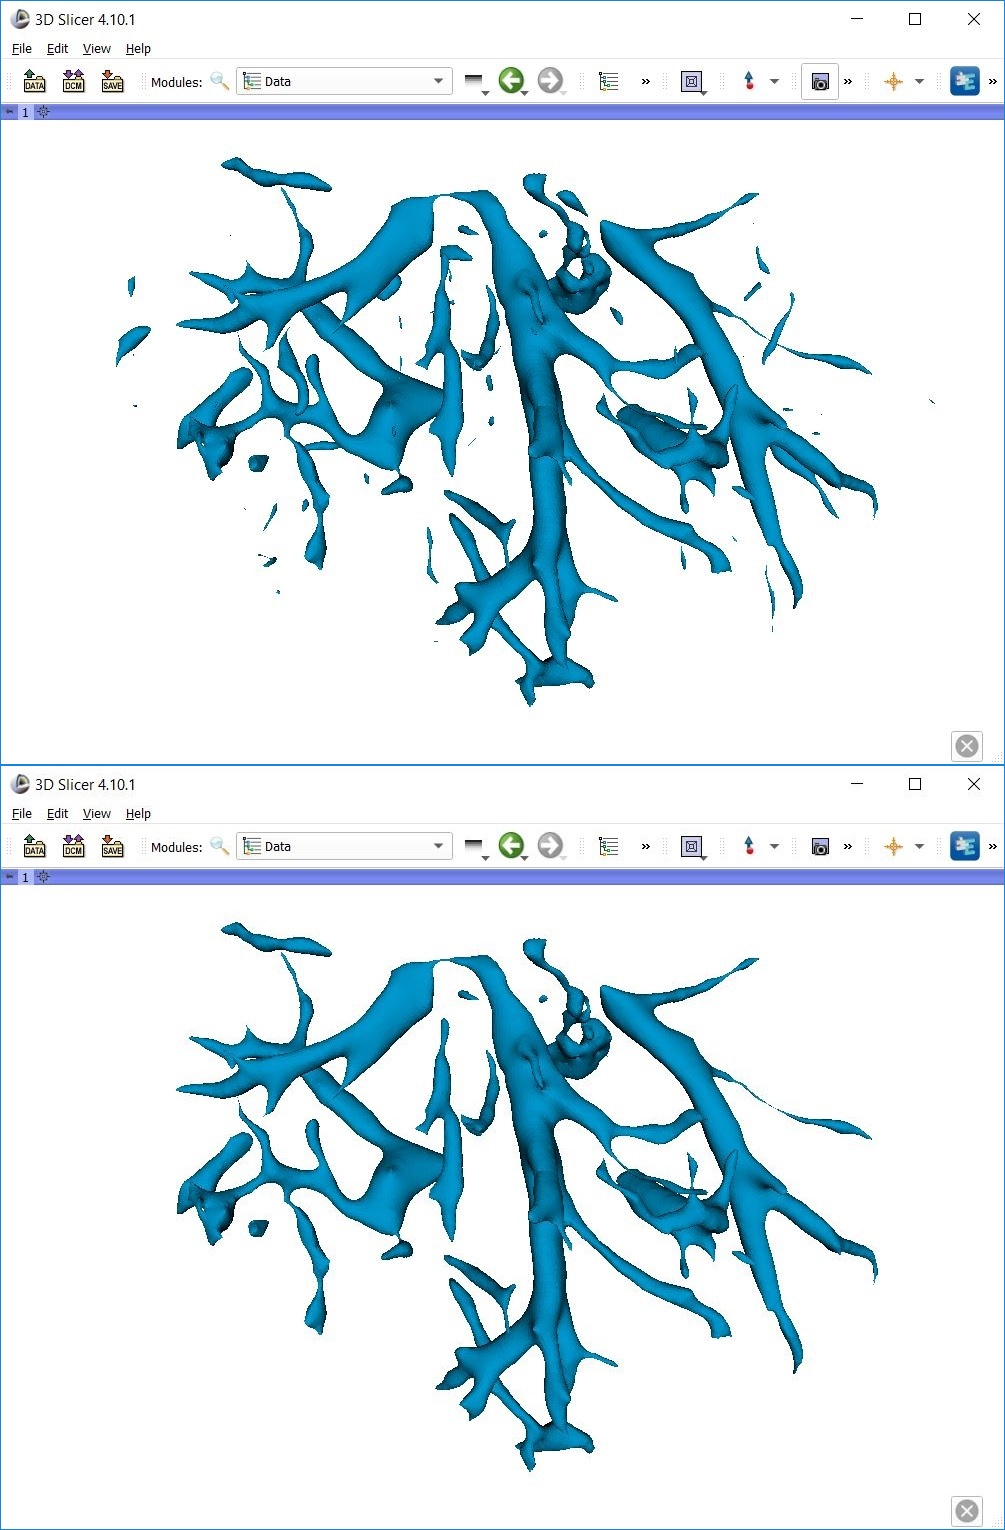
\includegraphics[width=\textwidth, height=.925\textheight]{figures/result_e2_best_prediction_post_processing}
		\caption[Kết quả hệ thống mạch máu của trường hợp tốt nhất trong thí nghiệm 2.]{Kết quả hệ thống mạch máu của trường hợp tốt nhất trong thí nghiệm 2 trước và sau hậu xử lý. Các thành phần nhỏ và rời rạc đã được loại bỏ.}
		\label{fig:result_e2_best_prediction_post_processing}
	\end{figure}
	\begin{figure}[h!]
		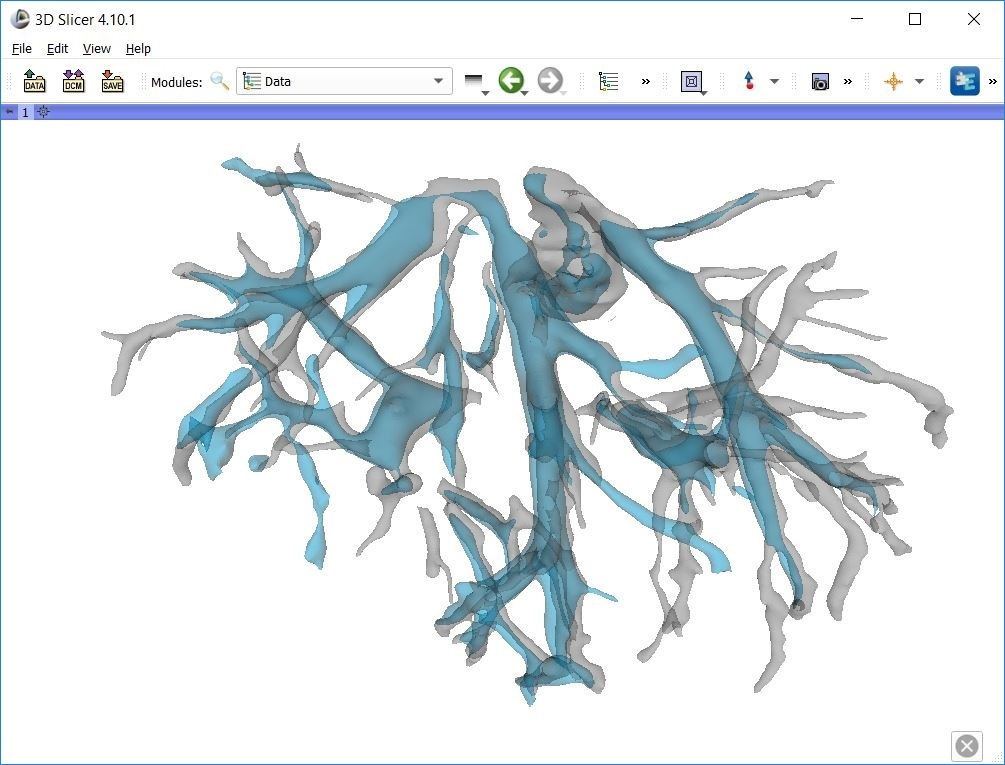
\includegraphics[width=\textwidth]{figures/result_e2_best_comparison}
		\caption[Kết quả hệ thống mạch máu của trường hợp tốt nhất trong thí nghiệm 2 và nhãn phân đoạn.]{Kết quả hệ thống mạch máu (màu xanh) của trường hợp tốt nhất trong thí nghiệm 2 khi so sánh với nhãn phân đoạn (màu xám). Hệ thống đã phân đoạn được các nhánh chính của mạch máu, tuy nhiên, còn rất nhiều nhánh mạch máu nhỏ hệ thống chưa phân đoạn được.}
		\label{fig:result_e2_best_comparison}
	\end{figure}
	\begin{figure}[h!]
		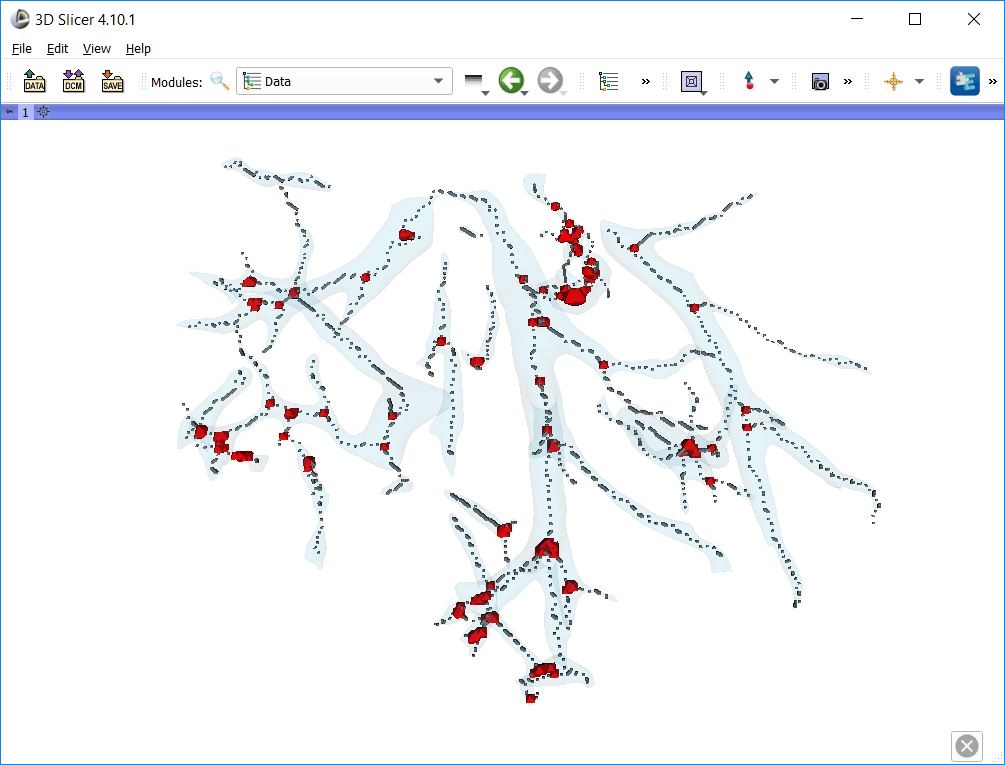
\includegraphics[width=\textwidth]{figures/result_e2_best_skeleton_branching_point}
		\caption[Kết quả tìm đường chính giữa và điểm phân nhánh của trường hợp tốt nhất trong thí nghiệm 2.]{Kết quả tìm đường chính giữa (đường màu xám) và điểm phân nhánh (màu đỏ) của trường hợp tốt nhất trong thí nghiệm 2. Hệ thống đã xác định được đường chính giữa và các điểm phân nhánh của mạch máu.}
		\label{fig:result_e2_best_skeleton_branching_point}
	\end{figure}


	\begin{figure}[h!]
		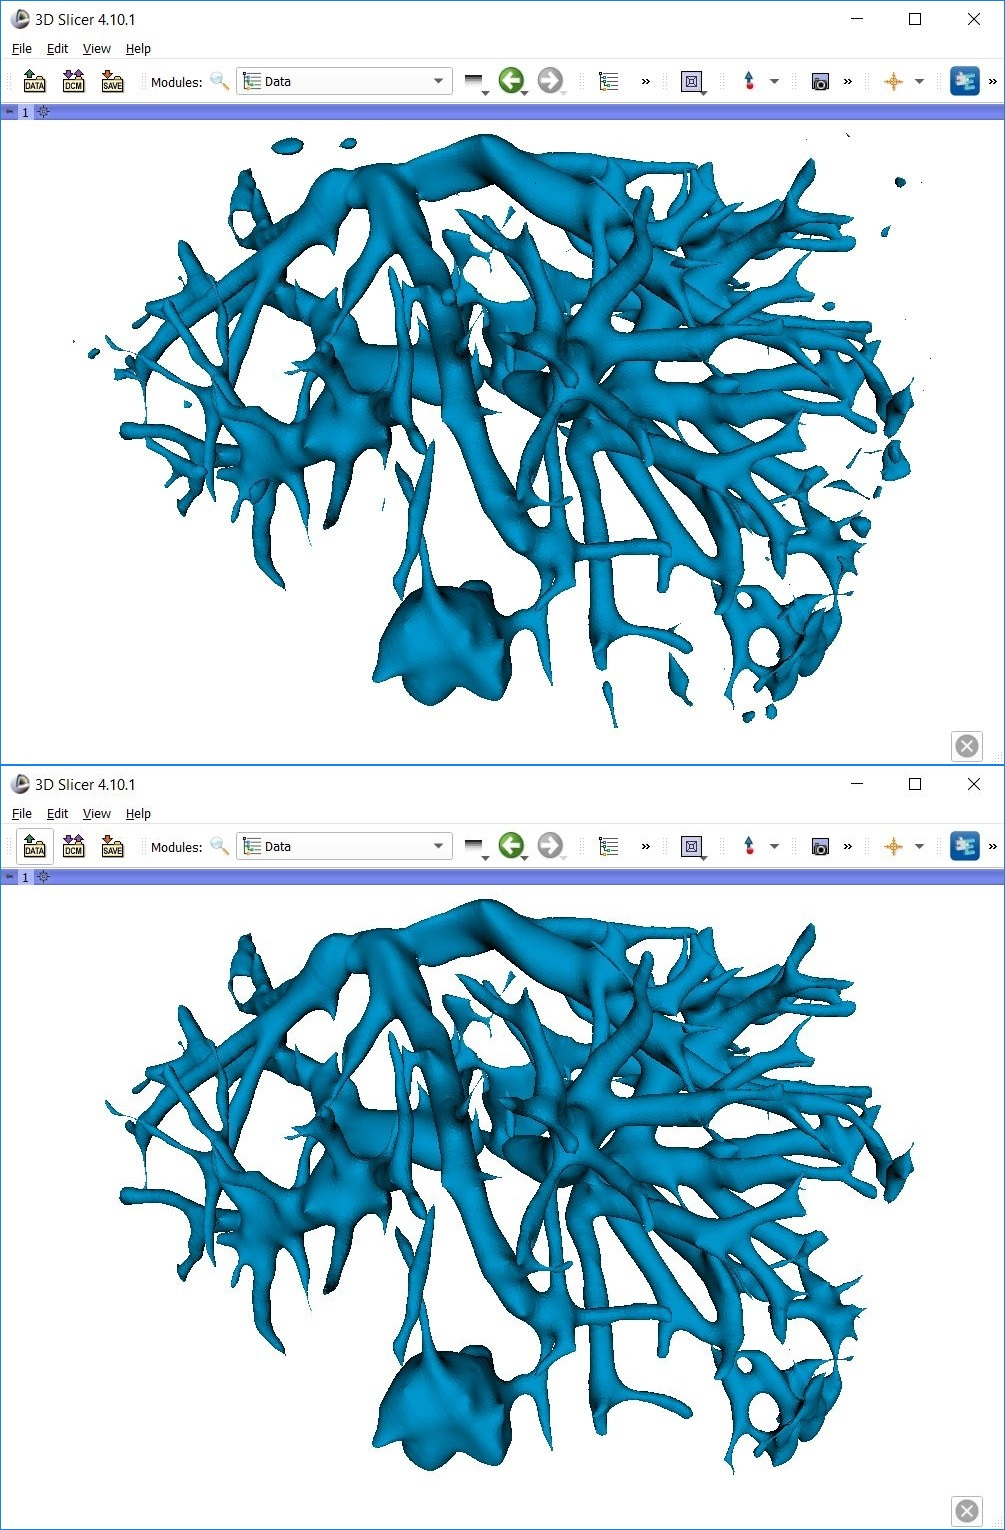
\includegraphics[width=\textwidth, height=0.925\textheight]{figures/result_e2_worst_prediction_post_processing}
		\caption[Kết quả hệ thống mạch máu của trường hợp xấu nhất trong thí nghiệm 2.]{Kết quả hệ thống mạch máu của trường hợp xấu nhất trong thí nghiệm 2 trước và sau hậu xử lý. Hệ thống phân đoạn mạch máu quá lớn, bước hậu xử lý không có nhiều hiệu quả.}
		\label{fig:result_e2_worst_prediction_post_processing}
	\end{figure}
	\begin{figure}[h!]
		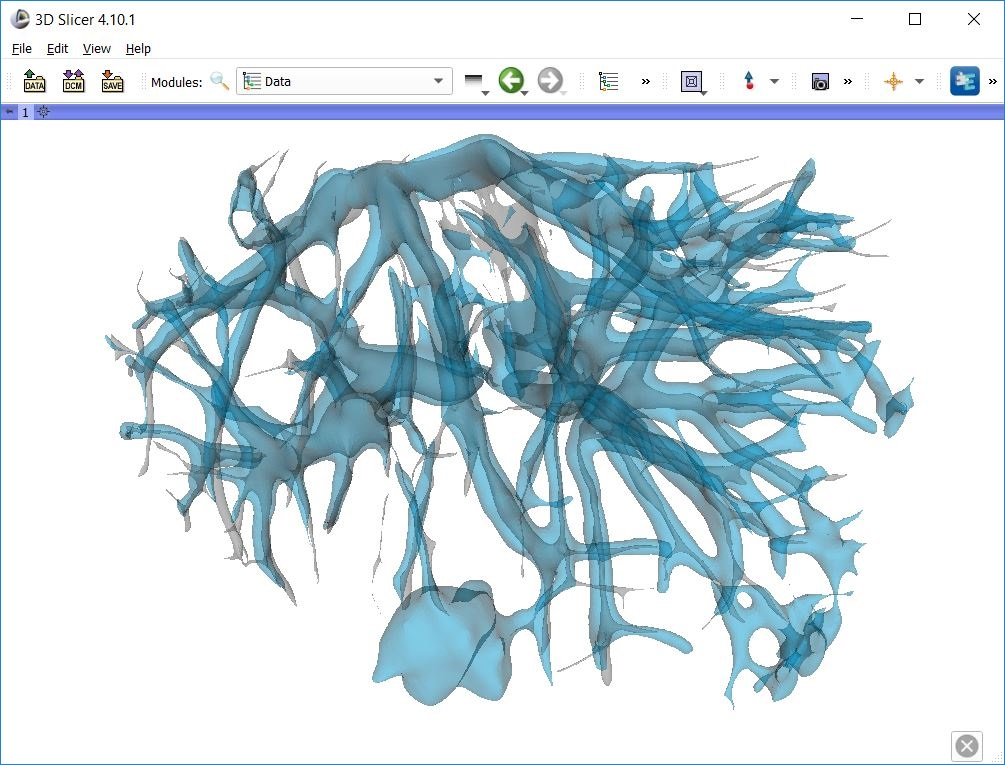
\includegraphics[width=\textwidth]{figures/result_e2_worst_comparison}
		\caption[Kết quả hệ thống mạch máu của trường hợp xấu nhất trong thí nghiệm 2 và nhãn phân đoạn.]{Kết quả hệ thống mạch máu (màu xanh) của trường hợp xấu nhất trong thí nghiệm 2 khi so sánh với nhãn phân đoạn (màu xám). Các mạch máu được phân đoạn lớn hơn rất nhiều so với thực tế. Ngoài ra, xuất hiện một khối phân đoạn sai rất lớn có thể là khối u.}
		\label{fig:result_e2_worst_comparison}
	\end{figure}
	\begin{figure}[h!]
		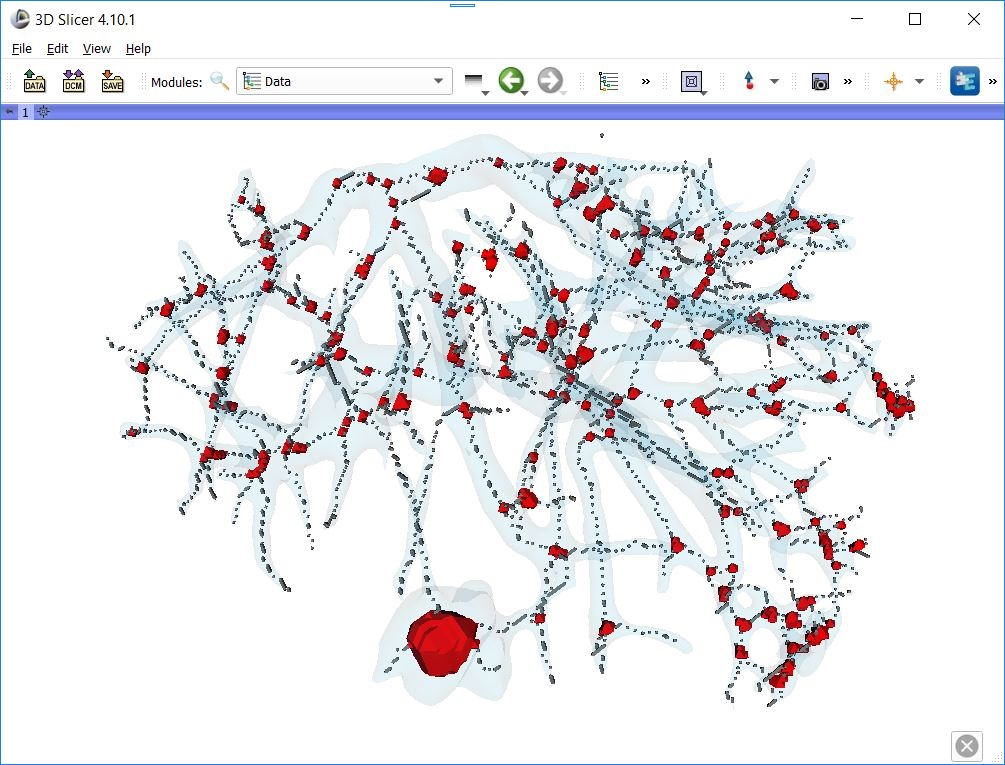
\includegraphics[width=\textwidth]{figures/result_e2_worst_skeleton_branching_point}
		\caption[Kết quả tìm đường chính giữa và điểm phân nhánh của trường hợp xấu nhất trong thí nghiệm 2.]{Kết quả tìm đường chính giữa (đường màu xám) và điểm phân nhánh (màu đỏ) của trường hợp xấu nhất trong thí nghiệm 2. Hệ thống đã xác định được đường chính giữa và các điểm phân nhánh của mạch máu. Tuy nhiên, xuất hiện rất nhiều điểm phân nhánh sai.}
		\label{fig:result_e2_worst_skeleton_branching_point}
	\end{figure}

	\begin{figure}[h!]
		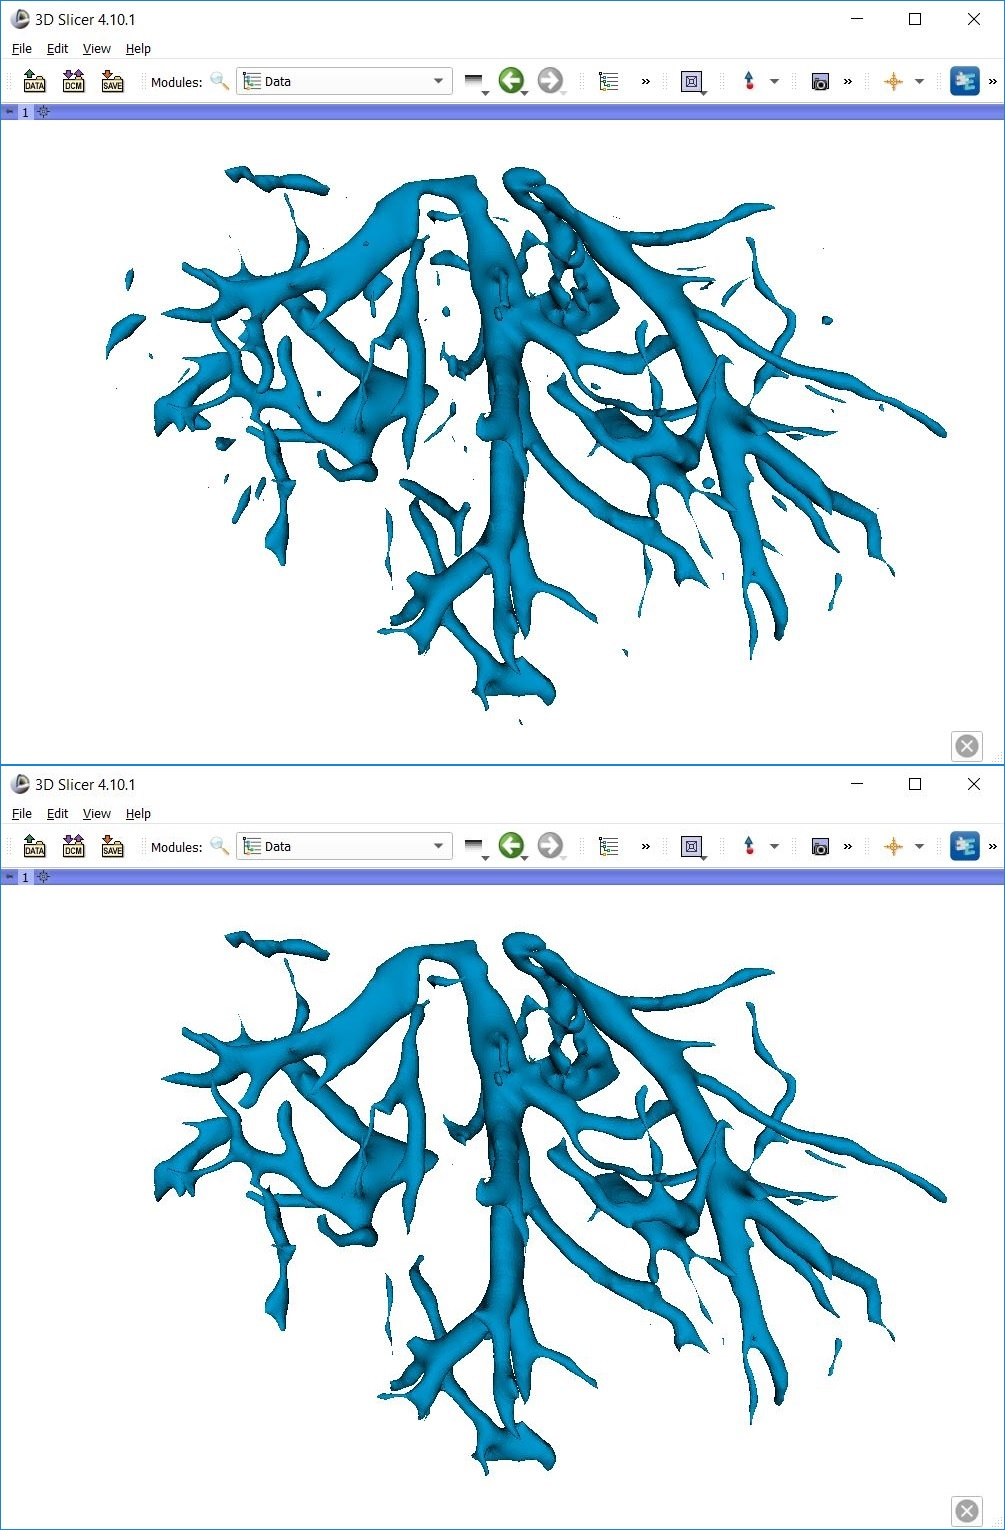
\includegraphics[width=\textwidth, height=0.925\textheight]{figures/result_e8_best_prediction_post_processing}
		\caption[Kết quả hệ thống mạch máu của trường hợp tốt nhất trong thí nghiệm 8.]{Kết quả hệ thống mạch máu của trường hợp tốt nhất trong thí nghiệm 8 trước và sau hậu xử lý. Các thành phần nhỏ và rời rạc hầu như đã được loại bỏ hoàn toàn.}
		\label{fig:result_e8_best_prediction_post_processing}
	\end{figure}
	\begin{figure}[h!]
		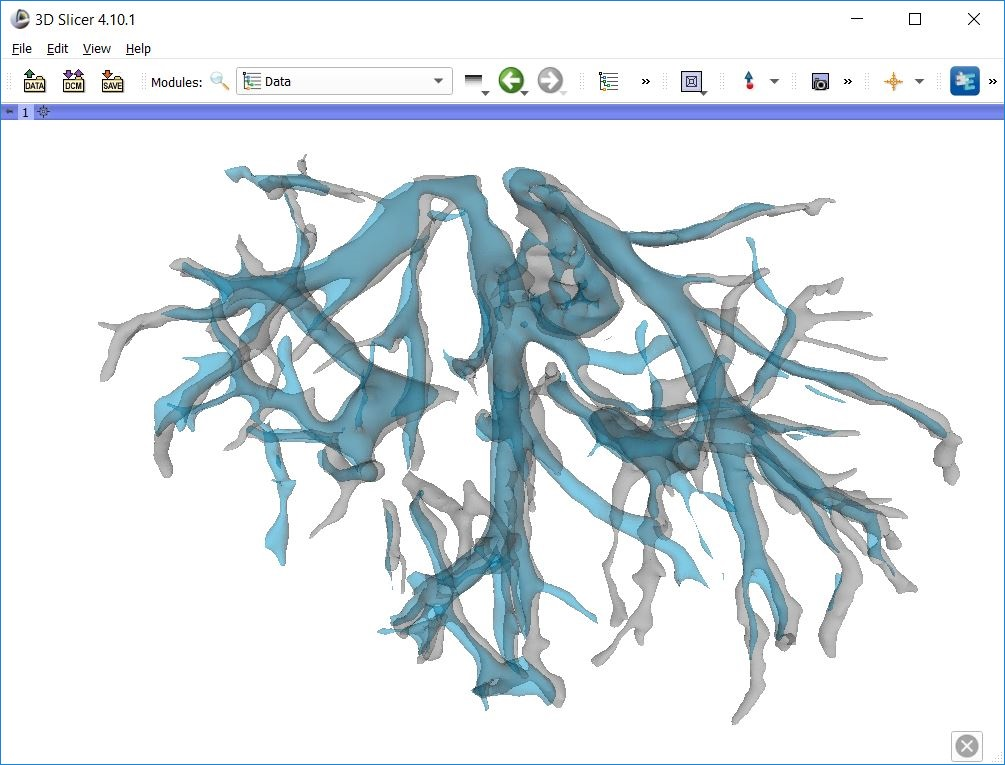
\includegraphics[width=\textwidth]{figures/result_e8_best_comparison}
		\caption[Kết quả hệ thống mạch máu của trường hợp tốt nhất trong thí nghiệm 8 và nhãn phân đoạn.]{Kết quả hệ thống mạch máu (màu xanh) của trường hợp tốt nhất trong thí nghiệm 8 khi so sánh với nhãn phân đoạn (màu xám). Kết quả phân đoạn khá sát với thực tế, chỉ một vài nhánh nhỏ chưa phân đoạn được.}
		\label{fig:result_e8_best_comparison}
	\end{figure}
	\begin{figure}[h!]
		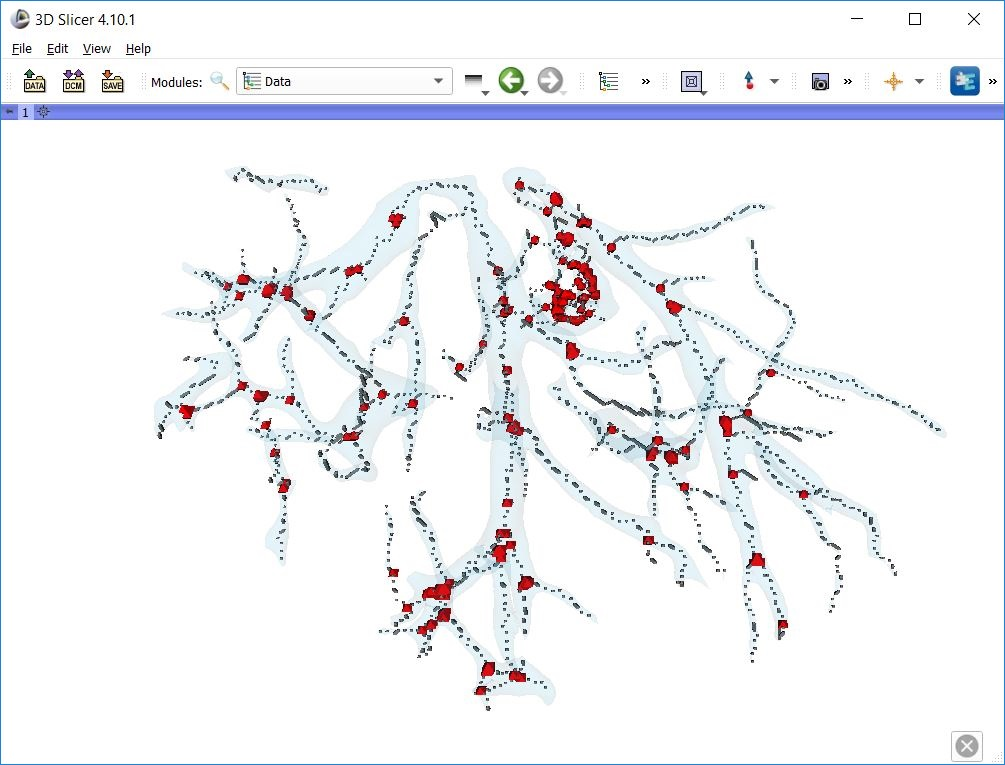
\includegraphics[width=\textwidth]{figures/result_e8_best_skeleton_branching_point}
		\caption[Kết quả tìm đường chính giữa và điểm phân nhánh của trường hợp tốt nhất trong thí nghiệm 8.]{Kết quả tìm đường chính giữa (đường màu xám) và điểm phân nhánh (màu đỏ) của trường hợp tốt nhất trong thí nghiệm 8. Hệ thống đã xác định được đường chính giữa và các điểm phân nhánh của mạch máu.}
		\label{fig:result_e8_best_skeleton_branching_point}
	\end{figure}
	\begin{figure}[h!]
		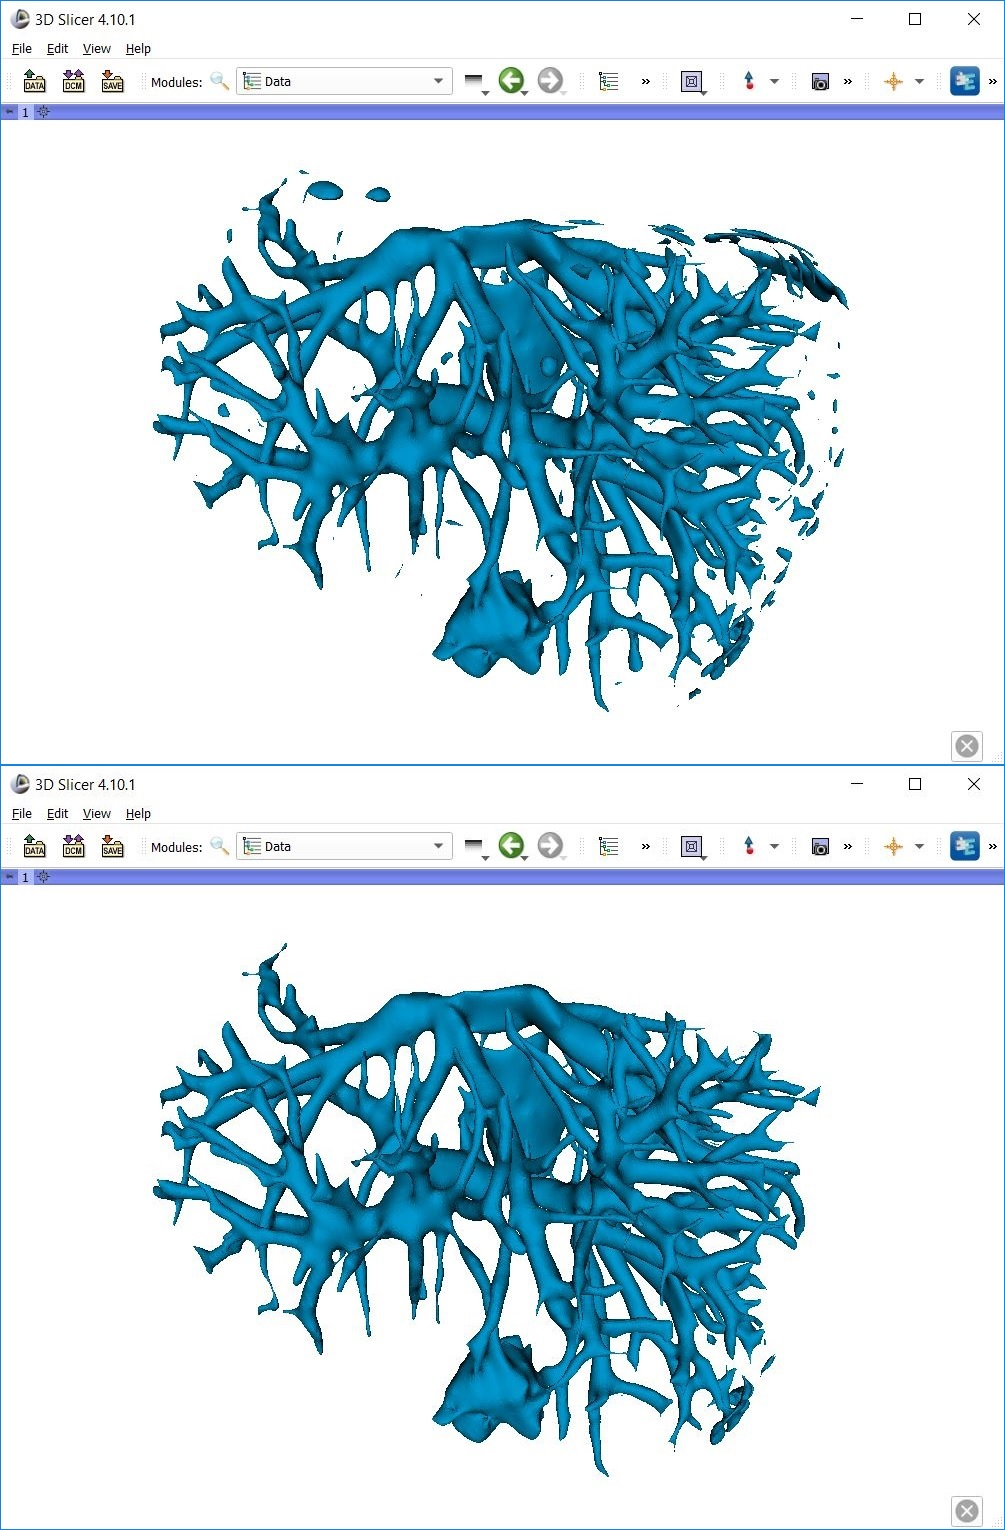
\includegraphics[width=\textwidth, height=0.925\textheight]{figures/result_e8_worst_prediction_post_processing}
		\caption[Kết quả hệ thống mạch máu của trường hợp xấu nhất trong thí nghiệm 8.]{Kết quả hệ thống mạch máu của trường hợp xấu nhất trong thí nghiệm 8 trước và sau hậu xử lý. Bước hậu xử lý đã loại bỏ đi rất nhiều vị trí dự đoán sai.}
		\label{fig:result_e8_worst_prediction_post_processing}
	\end{figure}
	\begin{figure}[h!]
		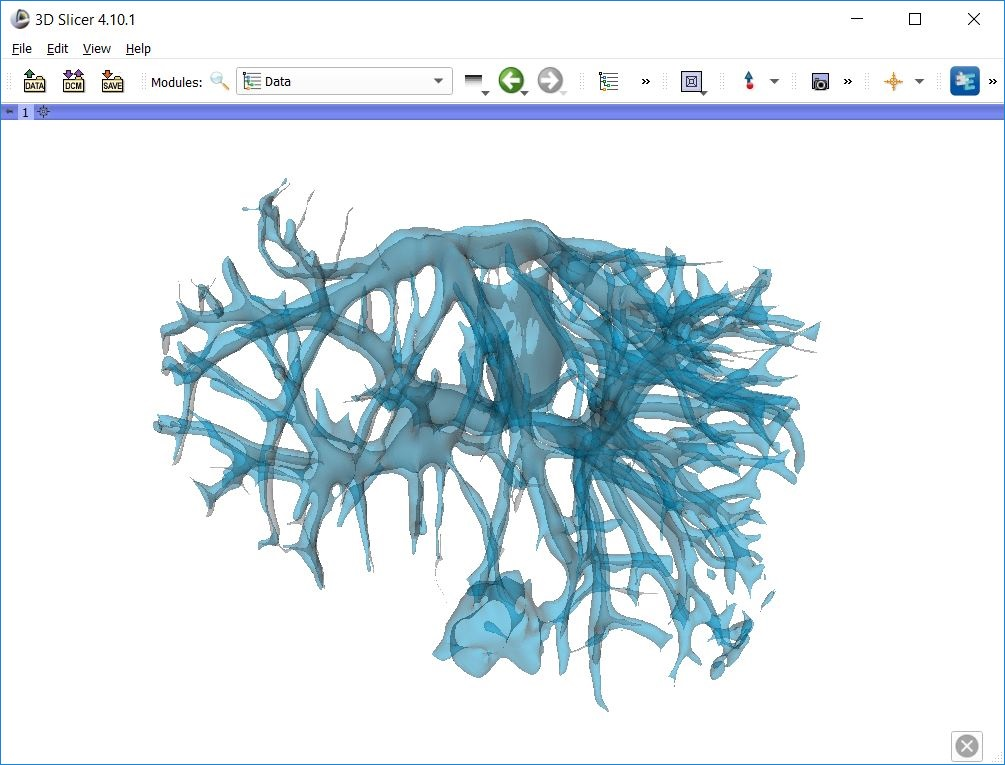
\includegraphics[width=\textwidth]{figures/result_e8_worst_comparison}
		\caption[Kết quả hệ thống mạch máu của trường hợp xấu nhất trong thí nghiệm 8 và nhãn phân đoạn.]{Kết quả hệ thống mạch máu (màu xanh) của trường hợp xấu nhất trong thí nghiệm 8 khi so sánh với nhãn phân đoạn (màu xám). Các mạch máu được phân đoạn lớn hơn rất nhiều so với thực tế. Ngoài ra, xuất hiện một khối phân đoạn sai rất lớn có thể là khối u.}
		\label{fig:result_e8_worst_comparison}
	\end{figure}
	\begin{figure}[h!]
		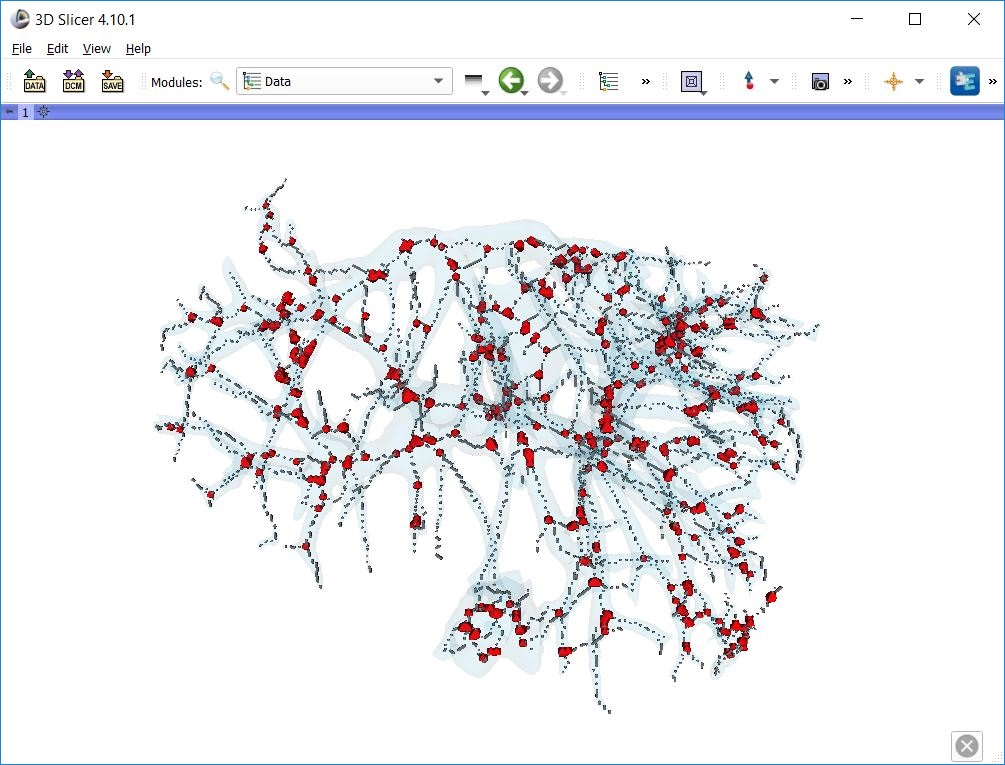
\includegraphics[width=\textwidth]{figures/result_e8_worst_skeleton_branching_point}
		\caption[Kết quả tìm đường chính giữa và điểm phân nhánh của trường hợp xấu nhất trong thí nghiệm 8.]{Kết quả tìm đường chính giữa (đường màu xám) và điểm phân nhánh (màu đỏ) của trường hợp xấu nhất trong thí nghiệm 8. Hệ thống đã xác định được đường chính giữa và các điểm phân nhánh của mạch máu. Tuy nhiên, xuất hiện rất nhiều đường chính giữa và điểm phân nhánh sai.}
		\label{fig:result_e8_worst_skeleton_branching_point}
	\end{figure}